%%%%%%%%%%%%%%%%%%%%%%%%%%%%%%%%%%%%%%%%%
%
% (c) 2022 by Jennifer Laaser
%
% This work is licensed under the Creative Commons Attribution-NonCommercial-ShareAlike 4.0 International License. To view a copy of this license, visit http://creativecommons.org/licenses/by-nc-sa/4.0/ or send a letter to Creative Commons, PO Box 1866, Mountain View, CA 94042, USA.
%
% The current source for these materials is accessible on Github: https://github.com/jlaaser/pogil-polymers
%
%%%%%%%%%%%%%%%%%%%%%%%%%%%%%%%%%%%%%%%%%

\renewcommand{\figpath}{content/polymchem/stepgrowth/Mn-and-stoich/figs}
\renewcommand{\labelbase}{Mn-and-stoich}

\begin{activity}{Degree of Polymerization in Step-Growth Polymerizations}
\label{\labelbase}

\begin{instructornotes}

	This activity introduces students to key concepts related to the degree of polymerization and stoichiometric balance in step-growth polymerizations.
	
	After completing this activity, students will be able to:
			\begin{enumerate}
				\item Calculate the number-average degree of polymerization for stoichiometrically-balanced step-growth polymerizations of `AB' or `AA+BB' monomer mixtures
				\item Explain what it means for a reaction to be stoichiometrically-balanced
				\item Describe the consequences of stoichiometric imbalance in terms of (a) the degree of polymerization and (b) the end-group functionality of the polymer chains.
			\end{enumerate}
	This activity will prepare students for follow-up activities on the chemistry, equilibria, kinetics, and molecular-weight distributions of step-growth polymerizations.
			
	\subsection*{Activity summary:}
	\begin{itemize}
		\item \textbf{Activity type:} Learning Cycle
		\item \textbf{Content goals:} See above
		\item \textbf{Process goals:} %https://pogil.org/uploads/attachments/cj54b5yts006cklx4hh758htf-process-skills-official-pogil-list-2015-original.pdf
			\begin{itemize}
				\item Analyzing data and extrapolating from a specific example to a general behavior
				\item Written and oral communication of reasoning
			\end{itemize}
		\item \textbf{Duration:} approx. 55 minutes including class discussion
		\item \textbf{Instructor preparation required:} none beyond knowledge of relevant content
		\item \textbf{Related textbook chapters:}
			\begin{itemize}
				\item \emph{Polymer Chemistry} (Hiemenz \& Lodge), 2nd ed.: sections 2.2 and 2.7
				\item \emph{Introduction to Polymers} (Young \& Lovell), 3rd ed.: section 3.2.3
			\end{itemize}
	\end{itemize}

\end{instructornotes}

	%\textbf{Focus question:} Put a central question for the students to consider through this exercise here.

\begin{model}[Polymerization of ``AB''-Type Monomers]
\label{\labelbase:mdl:ABpolym}

The simplest type of step-growth polymerization is one in which each monomer has one ``A''-type reactive group and one ``B''-type reactive group.
These types of monomers are referred to as ``AB''-type monomers.

In each step of the polymerization, an ``A'' group on one molecule reacts with a ``B'' group on another molecule to form an ``ab'' bond, as shown below:

\vspace{0.1in}
\centerline{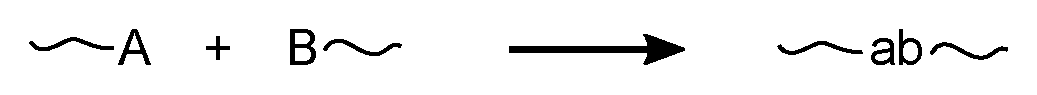
\includegraphics[width=0.6\textwidth]{\figpath/ABrxn.pdf}}

For example, for a simple reaction mixture containing 8 ``AB''-type monomers, the evolution of the reaction mixture might look something like this:

\vspace{0.1in}
\centerline{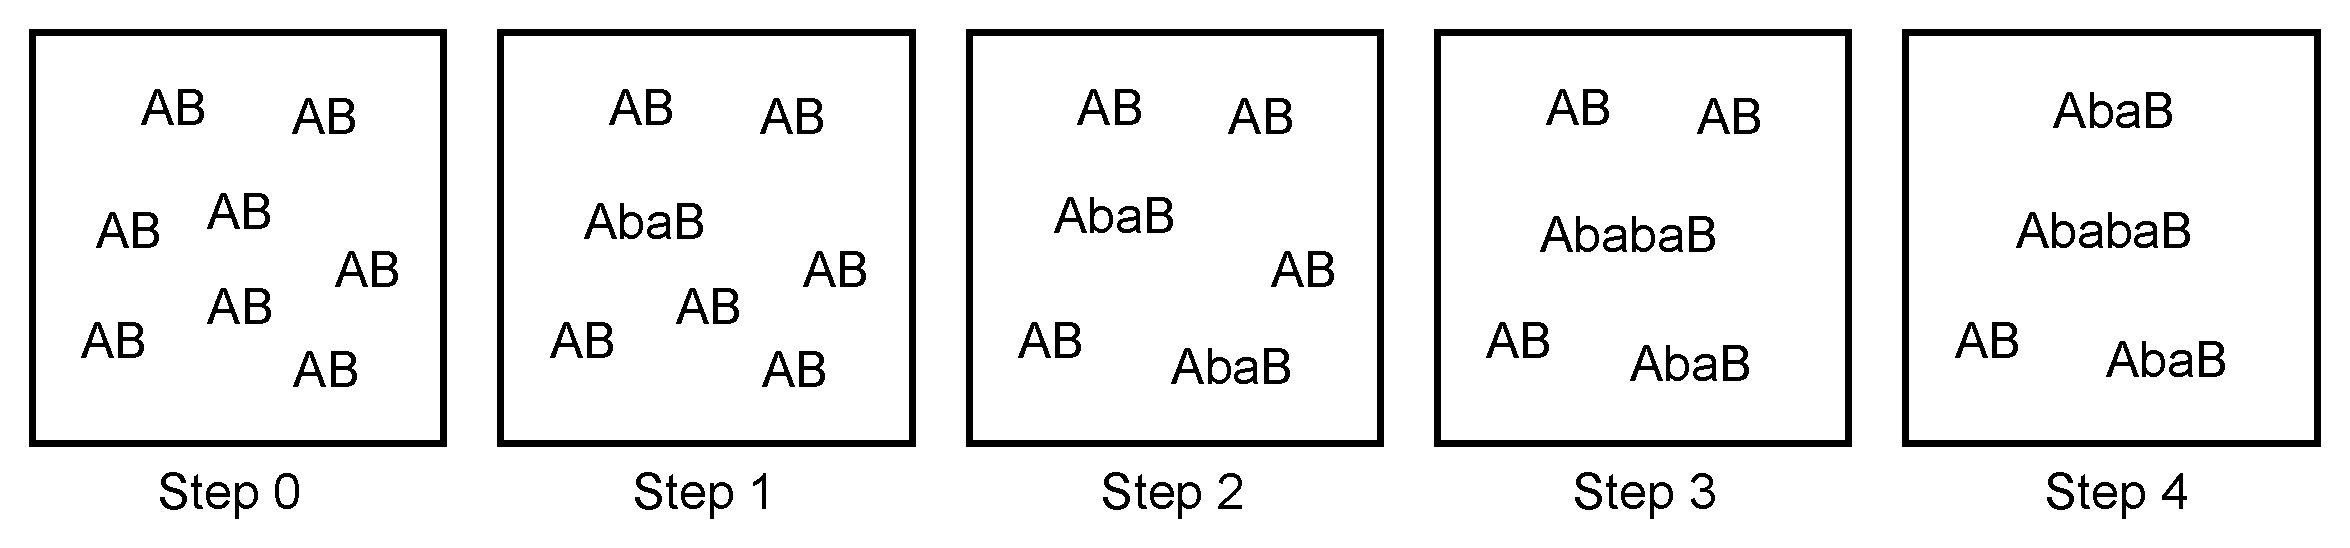
\includegraphics[width=0.9\textwidth]{\figpath/ABpolym.pdf}}

In this diagram, each string of letters represents one molecule; each molecule may be either an unreacted monomer (``AB'') or a growing polymer chain (e.g. ``AbaB'', ``AbabaB'', etc.).

\end{model}

\vspace{0.05in}
\begin{ctqs}

	\question \label{ctq:ABtable} Fill out the following table for the reaction mixture shown in Model \ref{\labelbase:mdl:ABpolym}:
	
			\begin{center}
				\renewcommand{\arraystretch}{3.25}
				\begin{tabular}{|c|c|c|}
					\hline
					\textbf{Step} &  \textbf{Number of unreacted ``A'' groups} & \textbf{Number of molecules} \\\hline
					0 & \answer{8} & \answer{8} \\\hline
					1 & \answer{7} & \answer{7}  \\\hline
					2 & \answer{6} & \answer{6}  \\\hline
					3 & \answer{5} & \answer{5}  \\\hline
					4 & \answer{4} & \answer{4}  \\\hline
				\end{tabular}
			\end{center}
		
	\question Explain, in a complete sentence, how the number of molecules in the mixture is related to the number of unreacted ``A'' groups.
		
		\begin{solution}[1in]{}
			The number of molecules in the mixture is exactly equal to the number of unreacted `A' groups at each step of the reaction.
		\end{solution}
		
\end{ctqs}

\begin{infobox}
At any given time, the number-average degree of polymerization, $N_n$, is the total initial number of \emph{monomers} divided by the  number of \emph{molecules} currently present.  That is,
\begin{equation*}
	N_n = \frac{\text{initial number of monomers}}{\text{current number of molecules}}
\end{equation*}
\end{infobox}

\vspace{0.05in}
\begin{ctqs}
		
		\question In Model \ref{\labelbase:mdl:ABpolym}, there were 8 monomers in the initial reaction mixture.  Using this information, calculate the number-average degree of polymerization for each step shown in Model 1.
		
			\begin{center}
				\renewcommand{\arraystretch}{4}
				\begin{tabular}{|c|c|c|c|c|c|}
					\hline
					\textbf{~~Step~~} &  \textbf{~~~~~0~~~~~} & \textbf{~~~~~1~~~~~} & \textbf{~~~~~2~~~~~} & \textbf{~~~~~3~~~~~} & \textbf{~~~~~4~~~~~} \\\hline
					$\mathbf{N_n}$ & \answer{8} & \answer{8/7=1.14} & \answer{8/6=1.33} & \answer{8/5=1.6} & \answer{8/4=2} \\\hline
				\end{tabular}
			\end{center}
		
		\question Suppose that you had initially started with 100 monomers.  Then, suppose that at some time later, you had only 8 unreacted ``A'' groups left.
		
			\begin{enumerate}
				\item How many molecules would there be in the reaction mixture at this point?
				
					\begin{solution}[0.75in]{}
						8
					\end{solution}
				
				\item What would the number-average degree of polymerization be at this point?
				
					\begin{solution}[0.75in]{}
						100/8 = 12.5
					\end{solution}
			\end{enumerate}
			
		\question \label{ctq:Nn-vA} More generally, suppose you started with $v_A^0$ monomers, and at some time later, you had only $v_A$ unreacted ``A'' groups left.  What would the number average-degree of polymerization be at this point, in terms of $v_A^0$ and $v_A$?
				
					\begin{solution}[0.75in]{}
						$N_n = \frac{v_A^0}{v_A}$
					\end{solution}
		
\end{ctqs}
	
\begin{infobox}

Usually, we find it more useful to work in terms of the \emph{fraction} of all ``A'' groups that have reacted, rather than the total \emph{number} of ``A'' groups that have reacted.

In step-growth polymerizations, we refer to the fraction of ``A'' groups that have reacted as the ``extent of reaction'', $p$.
When the fraction of ``A'' groups that \emph{have} reacted is $p$, the fraction of ``A'' groups that have \emph{not} reacted is $1-p$.

\end{infobox}
	
\begin{ctqs}
		
		\question \label{ctq:vA-p} If we start with $v_A^0$ ``A'' groups, what is $v_A$ (that is, how many ``A'' groups are still unreacted) when the extent of reaction is equal to $p$?
		
		\begin{solution}[1in]{}
			$v_A = (1-p)v_A^0$
			
			Note: students sometimes attempt to divide here, i.e. write $v_A = (1-p)/v_A^0$ or $v_A = v_A^0/(1-p)$. In the former case, ask them to think about the units on both sides of the equation.  In the latter case, ask them to think about whether it makes sense to have $v_A > v_A^0$.
		\end{solution}
		
		\question Using your answers to critical thinking questions \ref{ctq:Nn-vA} and \ref{ctq:vA-p}, derive an expression for $N_n$ in terms of $p$.
		
		\begin{solution}[1in]{}
			$N_n = \frac{v_A^0}{v_A} = \frac{v_A^0}{(1-p)v_A^0} = \frac{1}{1-p}$
		\end{solution}
		
\end{ctqs}

\clearpage
\begin{model}[Polymerization of ``AA'' and ``BB''-Type Monomers]
\label{\labelbase:mdl:AABBpolym}

Now, let's consider a slightly more complicated reaction, with two different types of monomers that each have \emph{either} two ``A'' reactive groups \emph{or} two ``B'' reactive groups.
We call monomers with two ``A'' groups ``AA''-type monomers, and we call monomers with two ``B'' groups ``BB''-type monomers.

Suppose we start with 8 monomers, 4 of which are ``AA''-type monomers and 4 of which are ``BB''-type monomers.
In this case, the evolution of the reaction mixture might look something like this:

\vspace{0.1in}
\centerline{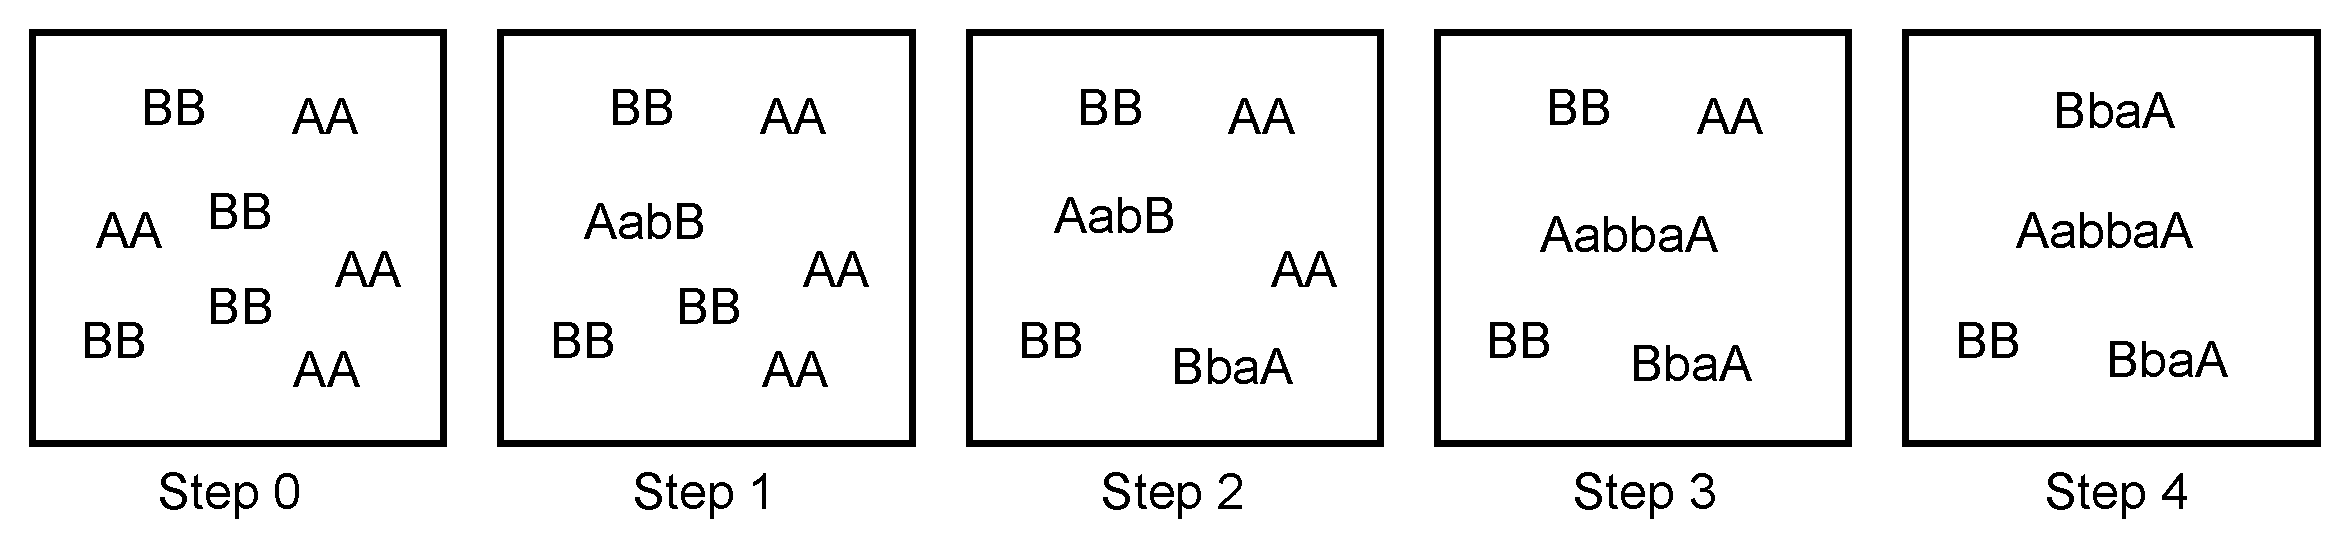
\includegraphics[width=0.9\textwidth]{\figpath/AABBpolym.pdf}}

\end{model}

\begin{ctqs}
		\question \label{ctq:AABBtable} For the reaction mixture shown in Model \ref{\labelbase:mdl:AABBpolym}, fill out the following table:
		
			\begin{center}
				\renewcommand{\arraystretch}{3}
				\begin{tabular}{|c|c|c|c|}
					\hline
					\textbf{Step} &  \textbf{Number of unreacted ``A'' groups} & \textbf{Number of molecules} & ~~~~$\mathbf{N_n}$~~~~\\\hline
					0 & \answer{8} & \answer{8} & \answer{8/8=1} \\\hline
					1 & \answer{7} & \answer{7} & \answer{8/7=1.14} \\\hline
					2 & \answer{6} & \answer{6} & \answer{8/6=1.33} \\\hline
					3 & \answer{5} & \answer{5} & \answer{8/5=1.6} \\\hline
					4 & \answer{4} & \answer{4} & \answer{8/4=2} \\\hline
				\end{tabular}
			\end{center}
			
		\question Compare your answers in CTQ \ref{ctq:AABBtable} with those from CTQ \ref{ctq:ABtable}.  What similarities and/or differences do you notice?
		
			\begin{solution}[1in]{}
				The numbers are exactly the same - the `AA+BB' reaction behaves exactly the same as the polymerization of `AB' monomers.
			\end{solution}
		
		\question Consider the following statement:
		
			\emph{``In polymerizations of AA- and BB-type monomers, we should be able to use the same expressions to calculate $N_n$ as we did for polymerizations of AB-type monomers.''}
			
			In two or three complete sentences, briefly critique or defend this statement, making sure to explain your reasoning.
		
			\begin{solution}[1.75in]{}
				DEFEND: In both types of polymerizations, one step of the reaction uses up one `A' reactive group and decreases the total number of molecules by one. Thus, in both types of reactions, the total number of molecules will always be equal to the number of unreacted `A' groups, so at the same extent of reaction $p$ we should have the same number of molecules and thus the same molecular weight regardless of the type of monomers we started with.
				
				Note: students sometimes anticipate the stoichoimetric balance problem and will choose to critique this statement on the grounds that it is not true if the initial numbers of A and B groups were not equal (or, that it is not true of the number of A groups is not equal to the initial number of molecules). 
			\end{solution}
			
\end{ctqs}
	
\begin{infobox}

A reaction is \emph{stoichiometrically balanced} if the initial reaction mixture contains exactly the same number of ``A'' and ``B'' reactive groups.

\end{infobox}
	
\begin{ctqs}
		\question Are the reactions in Models \ref{\labelbase:mdl:ABpolym} and \ref{\labelbase:mdl:AABBpolym} stoichiometrically balanced?  Briefly explain your answer in one or two complete sentences.
		
		\begin{solution}[1in]{}
			Yes, the reactions in Models \ref{\labelbase:mdl:ABpolym} and \ref{\labelbase:mdl:AABBpolym} are stoichiometrically balanced.  Both reactions start with 8 `A' functional groups and 8 `B' functional groups.  Since the number of `A' groups equals the number of `B' groups, the reactions are stoichiometrically-balanced.
		\end{solution}
		
		\question Predict what the reaction mixtures in Models \ref{\labelbase:mdl:ABpolym} and \ref{\labelbase:mdl:AABBpolym} might look like if you let them react until no more reactions could take place:
		
	\begin{solution}[2in]{\centerline{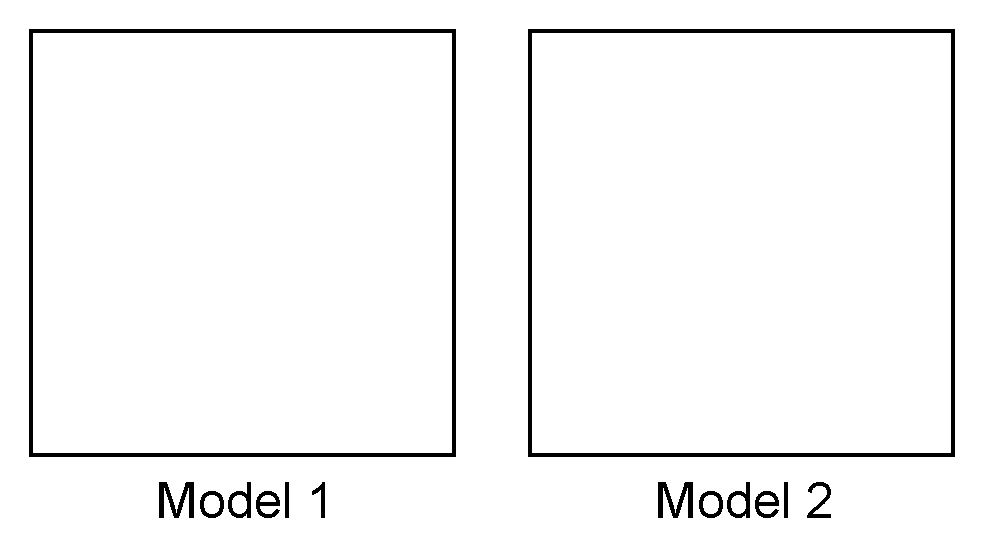
\includegraphics[width=0.6\textwidth]{\figpath/Model1and2_blank.pdf}}}
		\centerline{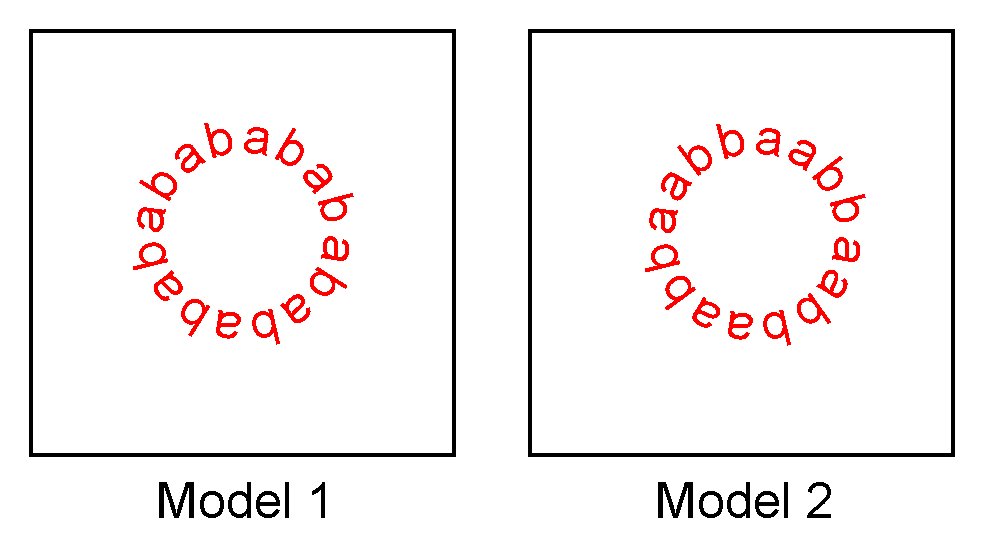
\includegraphics[width=0.4\textwidth]{\figpath/Model1and2_solution.pdf}}
		
		Note: many students may draw one linear chain with an unreacted `A' group on one end and an unreacted `B' group on the other. This answer will still give them the correct $N_n$, but is not strictly the product that would result if the system reacted until no more reactions can take place.  Ring formation may be worth a brief discussion since rings can be a side product in experimental step-growth polymerizations.
	
	\end{solution}
		
		\question Calculate the number-average degree of polymerization for both of the ``final'' states you drew in response to the previous question:
		
		\begin{solution}[1in]{}
			In both models, there is only one molecule in the final state.
			
			Thus, for both models, $N_n = 8/1 = 8$.
		\end{solution}
\end{ctqs}

\begin{model}[A Stoichiometrically-Imbalanced Reaction Mixture]
\label{\labelbase:mdl:stoichimbalance}

Practically speaking, it is often very difficult to ensure that a reaction mixture is perfectly stoichiometrically-balanced, and there is often a small excess of one type of monomer or the other.

In this model, consider a reaction mixture that starts with 3 AA-type monomers and 5 BB-type monomers:

\vspace{0.1in}
\centerline{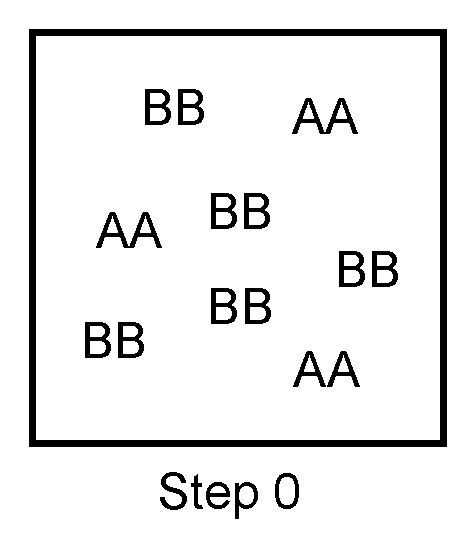
\includegraphics[width=0.4\textwidth]{\figpath/AABBpolym-nonstoich.pdf}}

\end{model}

\begin{ctqs}

		\question Fill in the blank spaces in the figure below with reasonable predictions for what the reaction mixture might look like in each successive step.
		
			\begin{solution}[1in]{\centerline{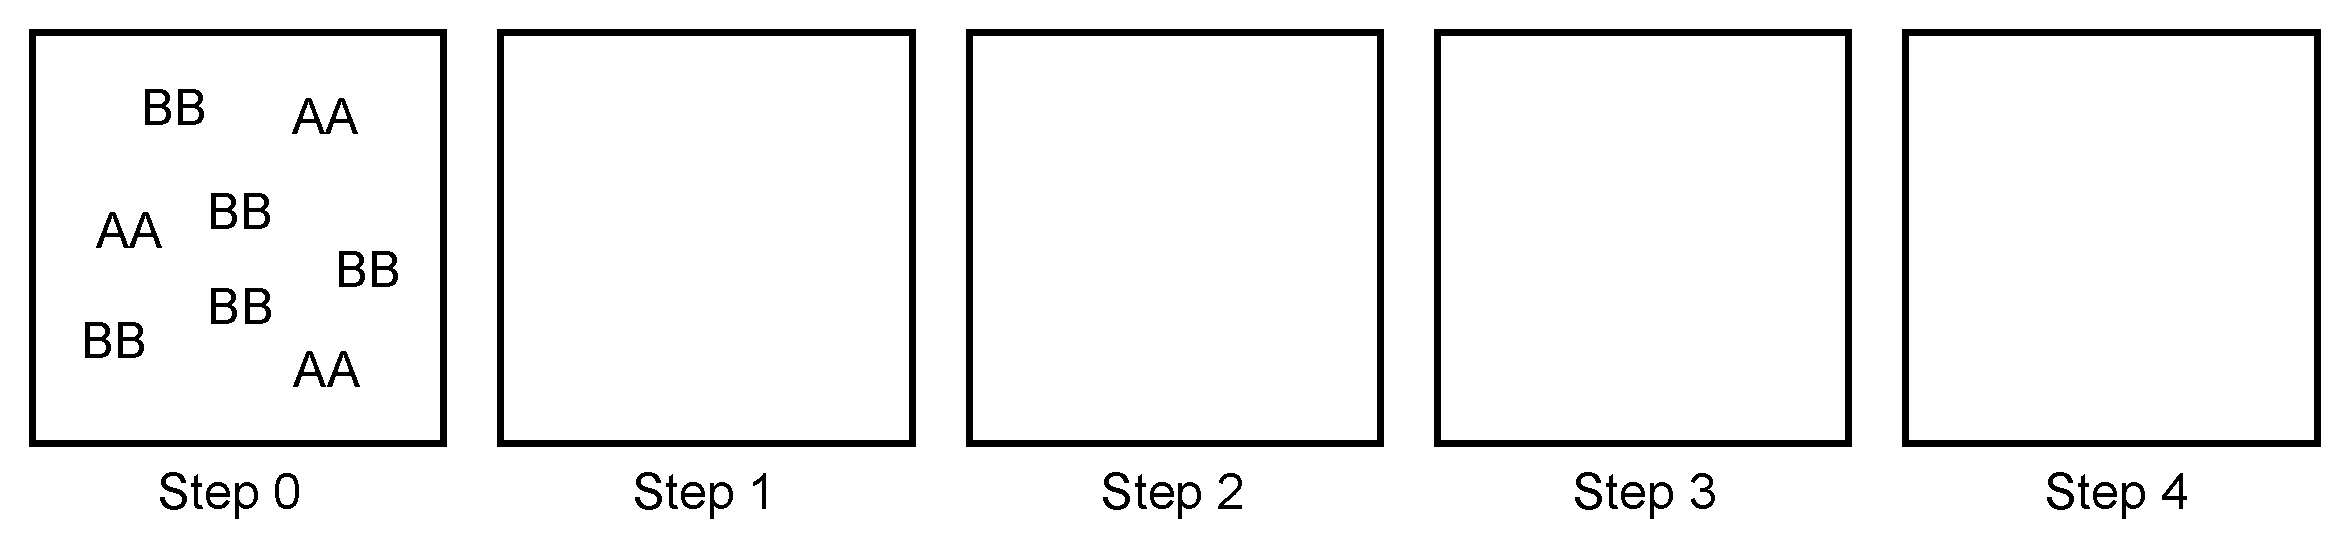
\includegraphics[width=0.9\textwidth]{\figpath/AABBpolym-nonstoichsteps_blank.pdf}}}
				\centerline{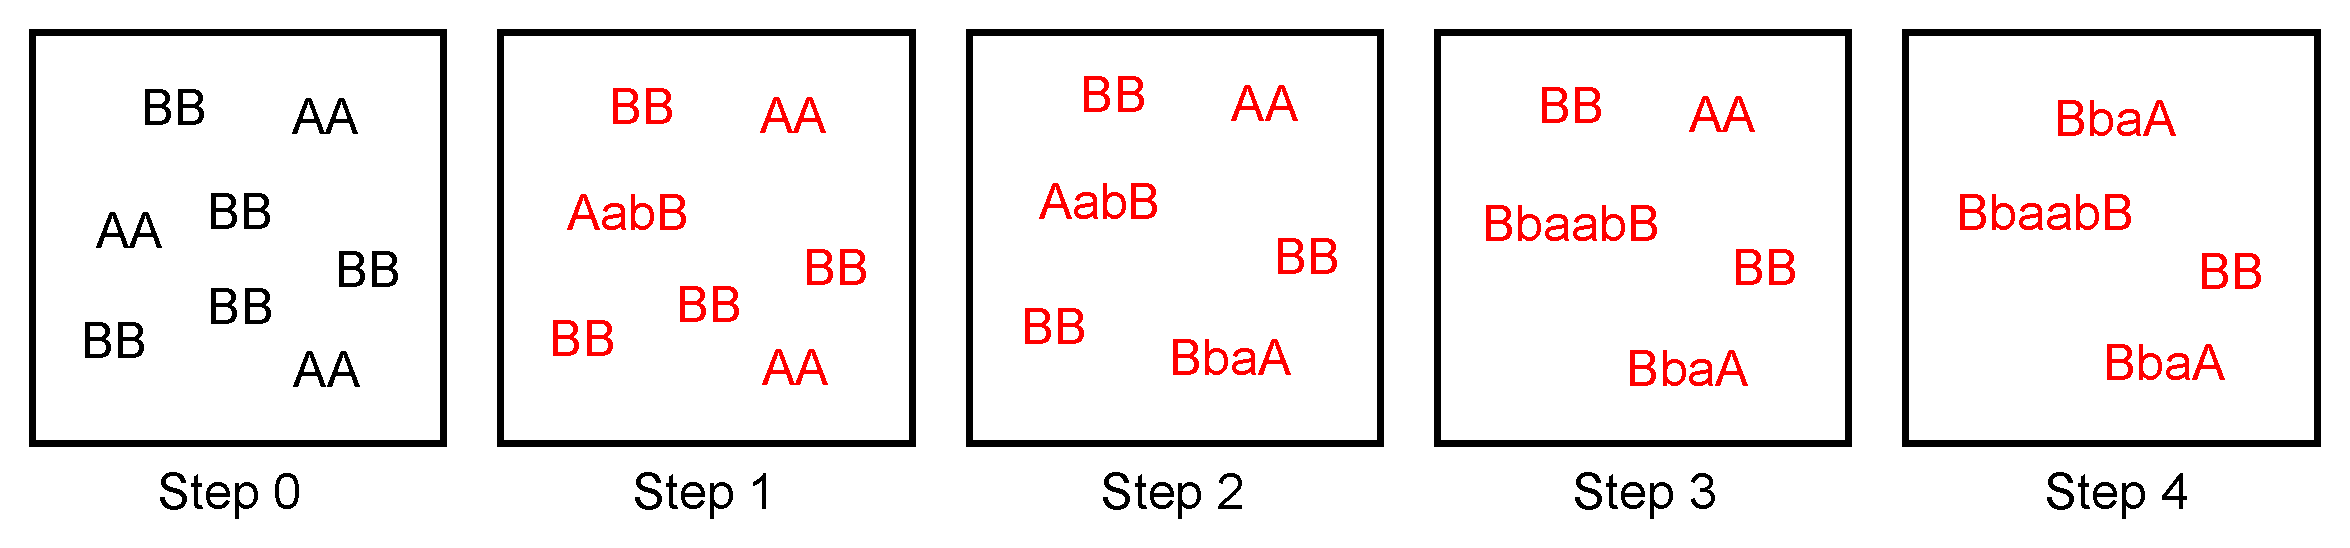
\includegraphics[width=0.9\textwidth]{\figpath/AABBpolym-nonstoichsteps_solution.pdf}}
			\end{solution}
		
		\clearpage
		\question Which type of reactive group is the ``limiting reagent'' in this reaction?  Briefly explain your reasoning.
		
			\begin{solution}[1in]{}
				Each step of the reaction uses up an equal number of `A' and `B' reactive groups. Since there are fewer `A' groups in the initial reaction mixture, the `A' reactive groups are the limiting reagent.
			\end{solution}
		
		\question \label{\labelbase:ctq:nonstoichpredict} Predict what the reaction mixture in Model \ref{\labelbase:mdl:stoichimbalance} might look like if you let it react until no more reactions could take place:
		
\begin{solution}[2in]{\centerline{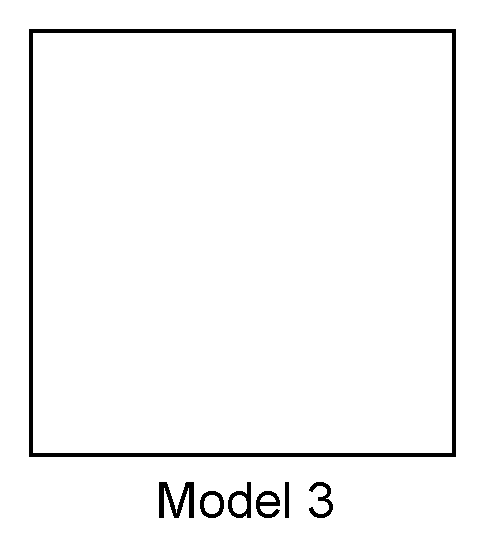
\includegraphics[width=0.3\textwidth]{\figpath/Model3_blank.pdf}}}
	\centerline{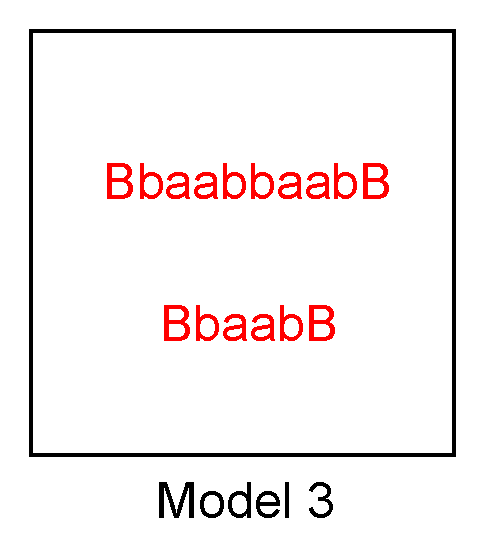
\includegraphics[width=0.3\textwidth]{\figpath/Model3_solution.pdf}}
\end{solution}
		
		\question Calculate the number-average degree of polymerization for the ``final'' state you drew in response to the previous question:
		
		\begin{solution}[1in]{}
			There are two molecules in the final reaction mixture, so the number-average degree of polymerization is $N_n = 8/2 = 4$.
		\end{solution}
		
		\question Is the final degree of polymerization for this stoichiometrically-unbalanced reaction smaller than, equal to, or larger than the final degree of polymerization you calculated for the stoichiometrically-balanced reactions in Models \ref{\labelbase:mdl:ABpolym} and \ref{\labelbase:mdl:AABBpolym}?
		
		\begin{solution}[1in]{}
			$N_n$ for the stoichiometrically-imbalanced reaction is \emph{smaller} than $N_n$ for the stoichiometrically-balanced reactions.
		\end{solution}
		
		\question Which type of reactive group is on the ends of all of the chains you drew in CTQ \ref{\labelbase:ctq:nonstoichpredict}?
		
		\begin{solution}[0.75in]{}
			All of the chains have `B' groups on the ends.
		\end{solution}
		
		\question Briefly critique or defend the following statement:
		
			\emph{``When drawing the structure of a polymer produced by a step-growth polymerization, we should always make sure that we draw end groups consistent with whichever reactive species was present in excess.''}
		
		\begin{solution}[1.85in]{}
		DEFEND: in a step growth polymerization, all of the molecules have either `A' groups or `B' groups on either end.  If there is an excess of `B' groups, the reaction will (ideally) go until all of the `A' groups have been used up, leaving only `B' groups on the ends of all of the polymer chains.
			
			Students may find an explicit example useful; one possibility is shown below:
			
			\centerline{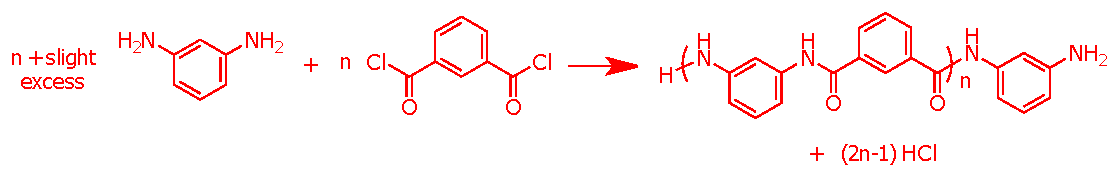
\includegraphics[width=0.8\textwidth]{\figpath/model3-endgrpexample}}			
			
			Here, the diamine is present in excess, so the polymer (Nomex) has amine groups on both ends.
		\end{solution}
			
\end{ctqs}
	
\begin{infobox}

In stoichiometrically-imbalanced step-growth polymerizations with an excess of B groups, we define a parameter $r$ that reflects the ratio of A groups to B groups.	
	If the initial number of A groups is $v_A^0$ and the initial number of B groups is $v_B^0$, then
	\begin{equation*}
		r = \frac{v_A^0}{v_B^0}
	\end{equation*}
	
	
	For a reaction mixture with stoichiometric imbalance $r$ at extent of reaction $p$, the number-average degree of polymerization is given by
	\begin{equation*}
		N_n = \frac{1+r}{1+r-2pr}
	\end{equation*}
	
\end{infobox}
	
\begin{ctqs}
		%\question When $r=1$, how can you simplify this expression for $N_n$?		
		%\question When $p=1$, how can you simplify this expression for $N_n$?
		\question Using this expression, fill in the following table with the expected number-average degree of polymerization for different combinations of $r$ and $p$ values:
		
			\begin{table}[!h]
				\centering
				\renewcommand{\arraystretch}{3}
				\begin{tabular}{|c|c|c|c|}
					\hline
					 &  ~$p=0.9$~ & ~$p=0.99$~ & ~$p=0.999$~ \\\hline
					$r=0.9$ & \answer{7} & \answer{16} & \answer{18.7} \\\hline
					$r=0.99$ & \answer{10} & \answer{67} & \answer{166} \\\hline
					$r=0.999$ & \answer{10} & \answer{95} & \answer{667} \\\hline
				\end{tabular}
			\end{table}
		
		\question On the basis of your answers to the previous question, briefly critique or defend the following statement:
		
			\emph{``Achieving high molecular weights in step-growth polymerizations requires both very precise measurement of the reagents, and reaction conditions which strongly favor the bond-forming reaction.''}
			
			\begin{solution}[2.5in]{}
				DEFEND: As we can see from the table in the previous question, achieving a large degree of polymerization requires \emph{both} $r$ and $p$ to be close to $1$.
				Since $r$ reflects the reagent ratio, this means that we must measure the reagents very precisely (and make sure they are as pure as possible!) to get as close to perfect stoichiometric balance as we can.
				Since $p$ reflects the extent of reaction, or the fraction of reactive groups that have reacted, getting $p$ close to 1 requires being able to push the $A+B\to ab$ reaction as far toward the products as possible.
			\end{solution}
			
\end{ctqs}

\begin{exercises}

		\exercise Often, when calculating extents of reaction and degrees of polymerization, our usual rules regarding significant figures don't work well.  To see why, do the following:  
		
			\begin{enumerate}
				\item Rearranging our equation for $N_n$ for a stoichiometrically-balanced reaction and solving for $p$, we find that $p = \frac{N_n-1}{N_n} = 1-\frac{1}{N_n}$.
				
					Using this equation, calculate the extent of reaction necessary to reach each of the following degrees of polymerization.  Write out as many digits as your calculator gives you.
				
			\begin{center}
				\renewcommand{\arraystretch}{3}
				\begin{tabular}{|c|c|}
					\hline
					$N_n$ &  ~~~~~~~~~~~~~~$p$~~~~~~~~~~~~~~ \\\hline
					10 & \answer{0.9} \\\hline
					100 & \answer{0.99} \\\hline
					300 & \answer{0.996666666...} \\\hline
					320 & \answer{0.996875} \\\hline
					1000 & \answer{0.999}  \\\hline
					10000 & \answer{0.9999} \\\hline
				\end{tabular}
			\end{center}
				
				\item How many significant figures are given in each of the $N_n$ values in the preceding problem?  What value(s) would you get for $p$ if you round your answer following the usual sig fig rules?
				
					\begin{solution}{}
							\emph{Most students} will likely apply the rule that the answer should be rounded to the same number of digits given in $N_n$.  In this case, they will conclude that:
						
							\begin{itemize}
								\item Each of the $N_n$ values in part (a) had exactly one significant figure, and
							
								\item rounding the calculated $p$ values to one sig-fig yields $p=0.9$ for $N_n=10$ and $p=1$ for all of the larger $N_n$ values.
							\end{itemize}
							
							\emph{Some students} may catch that since $p = 1-\frac{1}{N_n}$, $\frac{1}{N_n}$ should be have the same number of sig figs as given in $N_n$; since 1 is an exact number, putting it into the subtraction step as 1.00000000000$\dots$ then means that $p$ should be reported out to the decimal place corresponding to the last significant figure in $\frac{1}{N_n}$.  They will then answer as follows:
				
			\begin{center}
				\begin{tabular}{|c|c|c|c|}
					\hline
					$N_n$ & Number of sig figs & $\frac{1}{N_n}$ & $p=1.00000000\dots-\frac{1}{N_n}$ \\\hline
					10 & 1 & 0.1 & 0.9 \\\hline
					100 & 1 & 0.01 & 0.99 \\\hline
					300 & 1 & 0.003 & 0.997 \\\hline
					320 & 2 & 0.0031 & 0.9969 \\\hline
					1000 & 1 & 0.001 & 0.999  \\\hline
					10000 & 1 & 0.0001 & 0.9999 \\\hline
				\end{tabular}
			\end{center}
			
			where the two right-most columns have been rounded following the correct sig fig rules.
			
			However, in the author's experience, it is rare for students to catch this subtlety, and most will attempt to round directly to the number of sig figs given in $N_n$.
						
					\end{solution}
				
				\item In the context of your results, does the ``usual'' rule for sig figs make sense when calculating extents of reactions?  Explain  your reasoning in 1-2 complete sentences.
				
					\begin{solution}{}
							Students who rounded to the number of sig figs given in $N_n$ should answer \emph{no}: the usual sig fig rule for division, of rounding to the least number of sig figs present in the numbers going into the calculation, does not work, because it makes it impossible to distinguish extents of reaction corresponding to very different degrees of polymerization (ones that differ by several orders of magnitude or more!).
							
							Students who followed the more rigorous approach described above may answer \emph{yes}.
						
					\end{solution}
				
				\item Propose an alternate sig fig rule that would make more sense for calculating extents of reaction.
				
					\begin{solution}{}
							Student answers may vary.
							
							The most \emph{rigorous} answer is that if $N_n$ is given with $x$ significant figures, then $p$ should be reported with $x$ digits following the initial string of 9's.  For example, in the table given above, for $N_n=300$ (1 sig fig), $p$ should be reported as 0.997, while for $N_n = 320$ (2 sig figs), $p$ should be reported as 0.9969.  The exception is that when $N_n$ 10, 100, 1000, etc., the last 9 is the significant digit and no further digits should be reported.
							
							Conversely, when calculating $N_n$ from a given value for $p$, the number of significant figures in $N_n$ should be the number of digits following the leading string of 9's in $p$; if there are no digits following the leading string of 9's, then $N_n$ should be reported to one significant figure.
							
							Note that this rule follows directly from a rigorous treatment of the significant figures as described in the answer to part (b), above.
							
							The author has found that many students find this rule confusing, however, and has instead adopted the following simpler version in her classes: \emph{$p$ should be reported to the first digit that is not a 9}.
						
					\end{solution}
			\end{enumerate}

		\exercise In the stoichiometrically-balanced reactions in Models \ref{\labelbase:mdl:ABpolym} and \ref{\labelbase:mdl:AABBpolym}, the number of molecules was equal to the number of unreacted `A' groups in each step.  Is the same thing true for the stoichiometrically-imbalanced reaction in Model \ref{\labelbase:mdl:stoichimbalance}? Why or why not? % if not, how could you modify?
		
			\begin{solution}{}
				No, the same is not true for the stoichiometrically-imbalanced reaction in Model \ref{\labelbase:mdl:stoichimbalance}.  
				
				The key here is to realize that each step of the reaction does two things:
				\begin{enumerate}
					\item it uses up one `A' reactive group (and one `B' reactive group, but we're only counting `A' groups here)
					\item it decreases the total number of molecules in the reaction by one (it takes two molecules and links them together to form one)
				\end{enumerate}
				In Models \ref{\labelbase:mdl:ABpolym} and \ref{\labelbase:mdl:AABBpolym}, the stoichiometric balance means that the initial number of `A' groups is equal to the intial number of molecules.
				In each step, both of the number of unreacted `A' groups and the number of molecules decrease by one, so the number of `A' groups is always exactly equal to the number of molecules.
				
				In Model \ref{\labelbase:mdl:stoichimbalance}, however, the stoichiometric imbalance means that the initial number of `A' groups is smaller than the initial number of molecules.
				While the number of unreacted `A' groups and the number of molecules still both decrease by one in each step, they are not equal to each other since the initial values were not equal.
				
			\end{solution}
	
		\exercise In this activity, we only calculated the number-average \emph{degree of polymerization} of the polymers produced in step-growth polymerizations. However, usually, we want to be able to calculate the \emph{molecular weight} of the polymers as well.
		
			\begin{enumerate}
			
				\item In Model \ref{\labelbase:mdl:ABpolym}, we considered a reaction of AB-type monomers.  If each monomer had mass $m_{AB}$, how would you calculate the number-average molecular weight, $M_n$, of the polymer produced when the extent of reaction is equal to $p$?
				
					\begin{solution}{}
						Recall that, in general,
						\begin{equation*}
							M_n = M_0 N_n
						\end{equation*}
						where $M_0$ is the molecular weight of a single monomer and $N_n$ is the number of monomers.
						
						Here, the molecular weight of the monomer is $m_{AB}$, so
						\begin{equation*}
							M_n = m_{AB} N_n = \frac{m_{AB}}{1-p}
						\end{equation*}
					\end{solution}
				
				\item In Model \ref{\labelbase:mdl:AABBpolym}, we considered a stoichiometrically-balanced reaction of AA- and BB-type monomers. If the AA-type monomers each had mass $m_{AA}$ and the BB-type monomers each had mass $m_{BB}$, how would you calculate the number-average molecular weight of the polymer produced when the extent of reaction is equal to $p$?
				
					\emph{Note: this question is a little tricky - remember that $N_n$ counts \emph{monomers}, but in this reaction, not all of the monomers have the same molecular weight.  How might you be able to correct for this?}
					
					\begin{solution}{}
						To address this problem, we'll assume that on average, half of the monomers in each polymer chain will be AA-type monomers and half will be BB-type monomers (this is generally a reasonable assumption, except at very low degrees of polymerization).
						
						In this case, the average number of AA-type monomers in a given polymer chain is $N_n/2$, so their contribution to the molecular weight is $m_{AA}\frac{N_n}{2}$.  Similarly, the average number of BB-type monomers in a given polymer chain is also $N_n/2$, so their contribution to the molecular weight is $m_{BB}\frac{N_n}{2}$.
						
						Put together, the total molecular weight is
						\begin{align*}
							M_n &= m_{AA}\frac{N_n}{2} + m_{BB}\frac{N_n}{2}\\
								&= \frac{m_{AA} + m_{BB}}{2} N_n\\
								&= \frac{m_{AA} + m_{BB}}{2} \frac{1}{1-p}
						\end{align*}
						
						Note that the second line of this expression looks a lot like $M_n = M_0 N_n$, but with $M_0 = \frac{m_{AA} + m_{BB}}{2}$.  Thus, one way to interpret this result is to say that the number-average molecular weight is the number-average degree of polymerization times the \emph{average} molecular weight of the monomers.
					\end{solution}
				
			\end{enumerate}
		
		\exercise In Model \ref{\labelbase:mdl:stoichimbalance}, we considered a stoichiometrically-imbalanced reaction of AA- and BB-type monomers.  However, another important limit occurs when we have equal numbers of AA- and BB-type monomers, but add in an extra monofunctional reagent ``Bx'' that can only react on one side.
		
			In this exercise, suppose that we have $v_A^0$ `A' groups from AA-type monomers, $v_B^0$ `B' groups from BB-type monomers, and $v_{B'}^0$ `B' groups from Bx-type molecules.
		
			\begin{enumerate}
				\item Consider the following statements from two students:
					
					\begin{itemize}
				
					\item \textbf{Student 1:} \emph{``The total number of `B' groups is just $v_B^0 + v_{B'}^0$, so we can account for the presence of monofunctional Bx molecules by replacing $r=\frac{v_A^0}{v_B^0}$ with $r'=\frac{v_A^0}{v_B^0 + v_{B'}^0}$.''}
					
					\item \textbf{Student 2:} \emph{``One Bx molecule has the same effect on the degree of polymerization as one BB-type molecule.  Since Bx-type molecules have the same effect with half as many `B' groups, that means that a `B' group from a Bx molecule is twice as effective at stopping chain growth as a `B' group from a BB molecule, so we should replace $r$ with $r'=\frac{v_A^0}{v_B^0 + 2v_{B'}^0}$.''}
					\end{itemize}
					
					Which student do you agree with, and why?
				
					\begin{solution}{}
						Student 2 is correct.  Because extra BB-type and Bx-type molecules both effectively terminate a chain end and stop it from growing, one Bx-type molecule has the same effect on the degree of polymerization as one BB-type molecule.  As a result, the individual `B' groups in the BB-type molecule are essentially half as effective as the single `B' group in the Bx-type molecule, or, conversely, the `B' group in the Bx molecule is twice as effective as each `B' group from the BB-type molecules.
						
						One way to see this is to consider the simple reaction of one AA molecule with two Bx molecules.  In this case, when the reaction has gone all the way to completion, we should get a `xbaabx' oligomer.  This is essentially the same result that we would get from a reaction of one AA molecule with two BB molecules, which would result in a 'BbaabB' oligomer.  In both cases we end up with the same final degree of polymerization, even though we had twice as many `B' groups in the second case.
						
					\end{solution}
				
				\item Monofunctional reagents are a common impurity in supplies of difunctional monomers. Briefly explain why this means it is necessary to rigorously purify the starting materials used in step-growth polymerizations.
				
					\begin{solution}{}
						As seen above, monofunctional molecules are very effective at capping polymer chains and preventing the reaction from going further.  In a stoichiometrically-balanced reaction, if even just 5\% of the `B' groups come from monofunctional reagents, the average degree of polymerization will be capped at about 40 monomers, which is too short to be of much use in practical applications.  Rigorously purifying the reagents to remove monofunctional impurities is thus critical for achieving molecular weights high enough for most practical applications.
					\end{solution}
			\end{enumerate}
\end{exercises}
	
\end{activity}